\subsection{DAQ efficiency}
\begin{figure}[htbp]
  \centering
  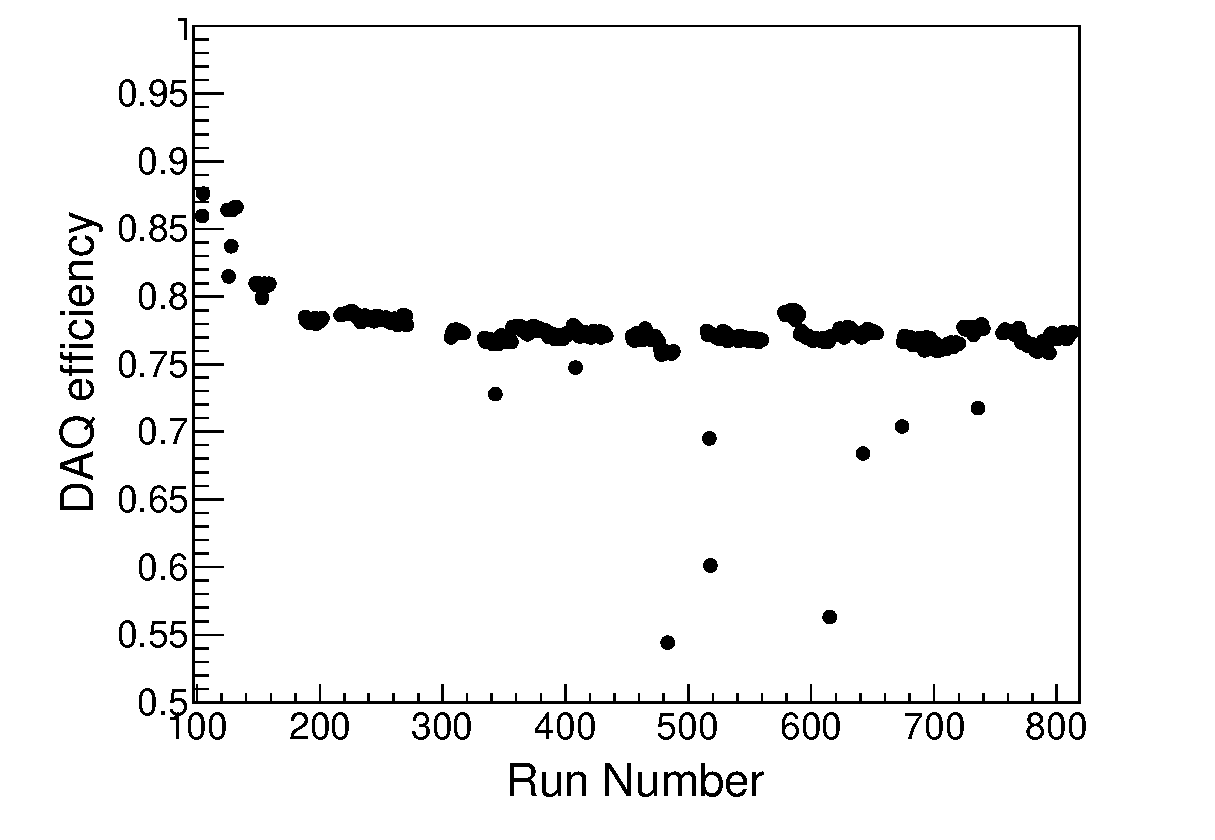
\includegraphics[width=8cm]{../pic/Run78/trigger/DAQ.eps}
  \caption{
    This figure shows DAQ live rate of production run in MR-RUN79.
  }
  \label{fig:DAQ_eff}
\end{figure}



When the DAQ system starts collecting data with a trigger signal, there is dead time for data conversion and transfer.
The signal for this is output from the VME SMP as the Computer busy signal, which is combined with the first level trigger signal as a veto.
Since no data is collected during dead time, its efficiency must be evaluated (DAQ efficiency).
The DAQ efficiency evaluates comparing numbers of trigger signal with and without the Computer busy signal.
Fig.\ref{fig:DAQ_eff} shows the DAQ efficiency of MR-RUN79.xs

\subsection{Trigger efficiency}
\begin{figure}[htbp]
  \centering
  \begin{tabular}{cc}
    \begin{minipage}{0.5\hsize}
      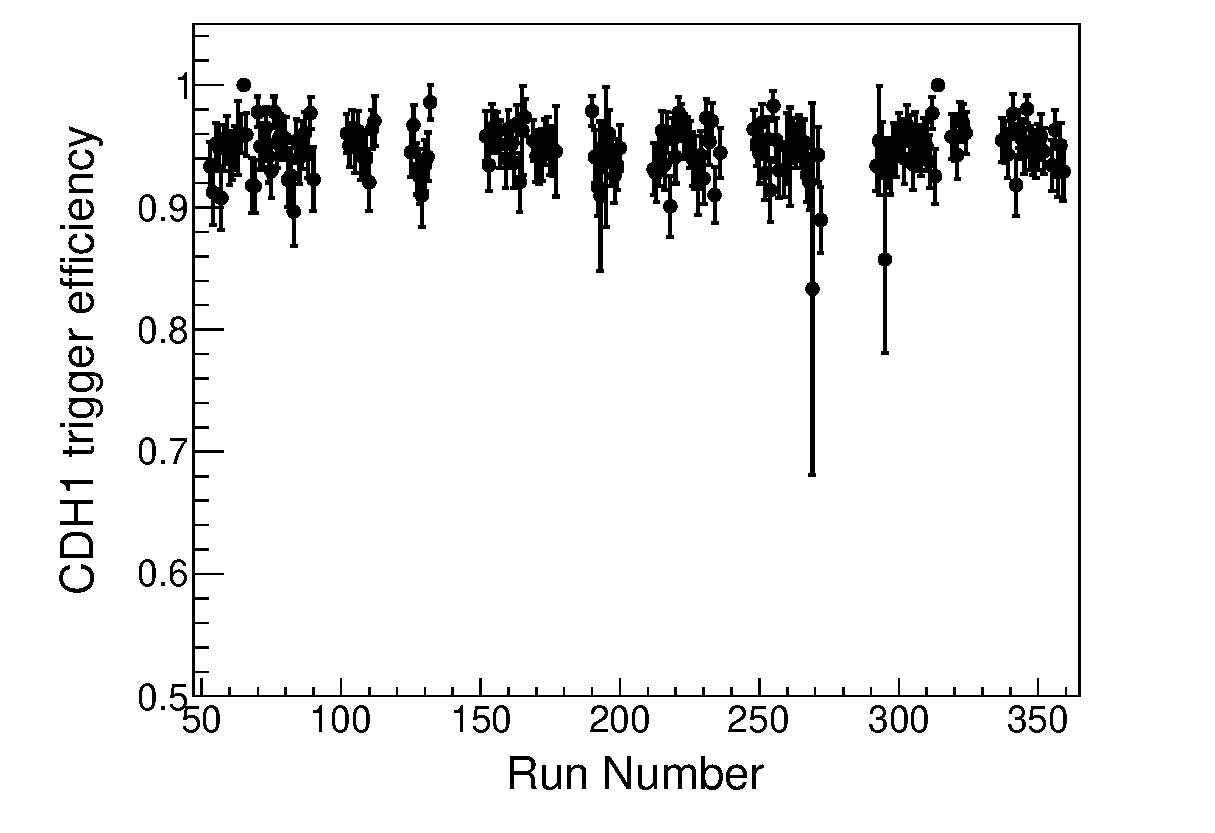
\includegraphics[width=5cm]{../pic/Run68/trigger/CDH1.eps}
    \end{minipage}

    \begin{minipage}{0.5\hsize}
      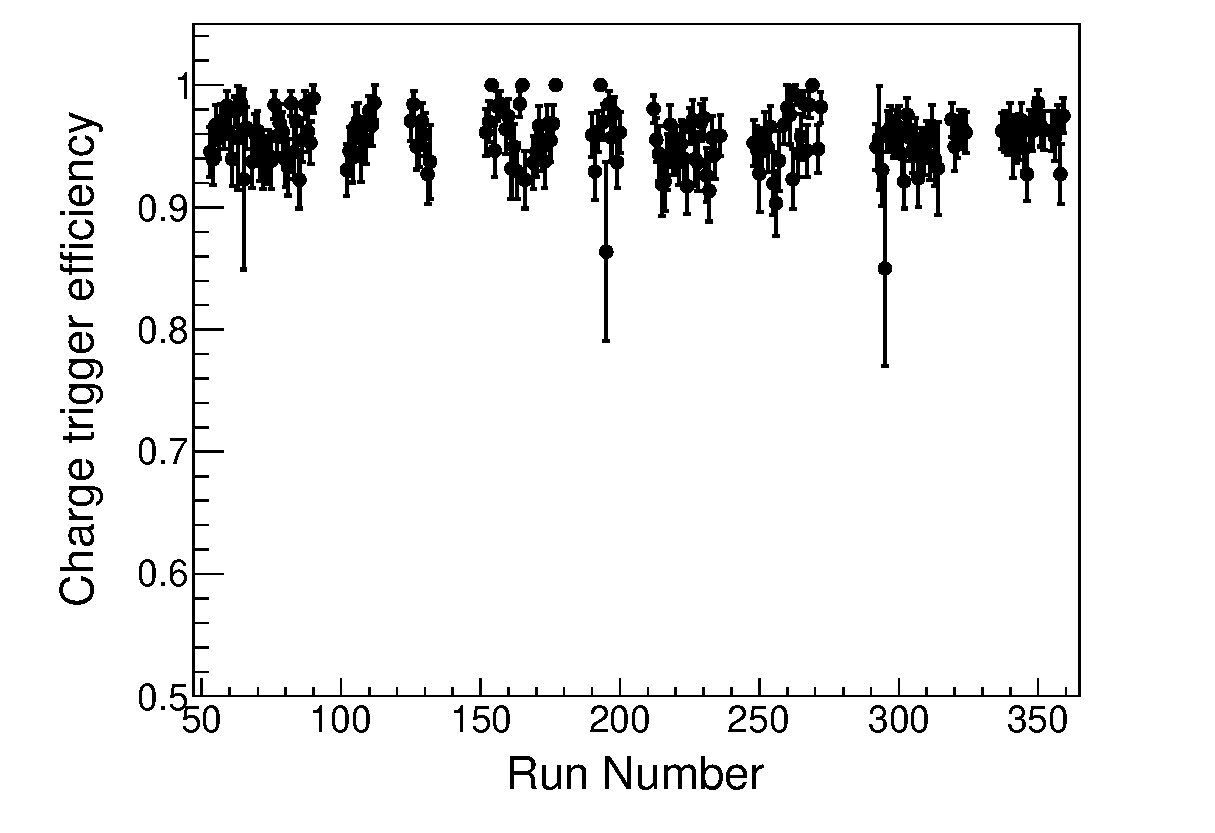
\includegraphics[width=5cm]{../pic/Run68/trigger/Charge.eps}
    \end{minipage}
  \end{tabular}

  \begin{tabular}{cc}
    \begin{minipage}{0.5\hsize}
      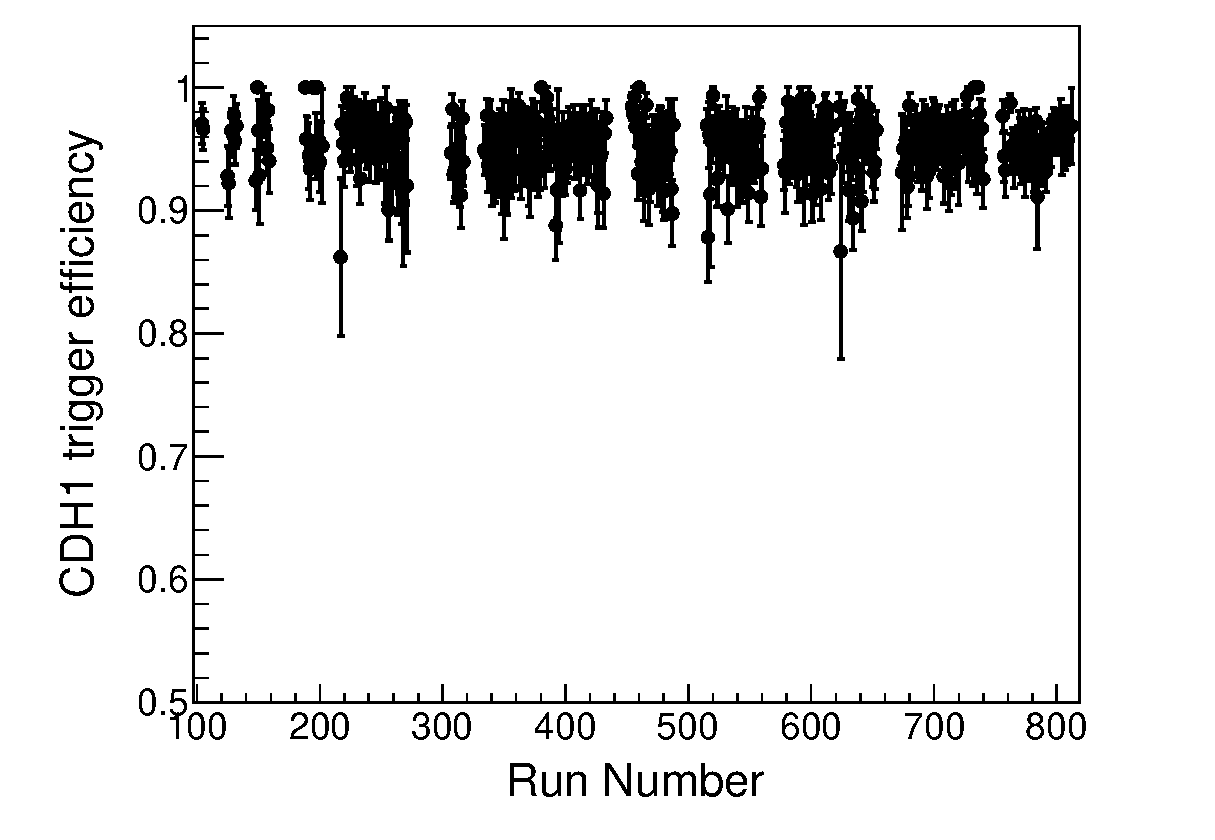
\includegraphics[width=5cm]{../pic/Run78/trigger/CDH1.eps}
    \end{minipage}

    \begin{minipage}{0.5\hsize}
      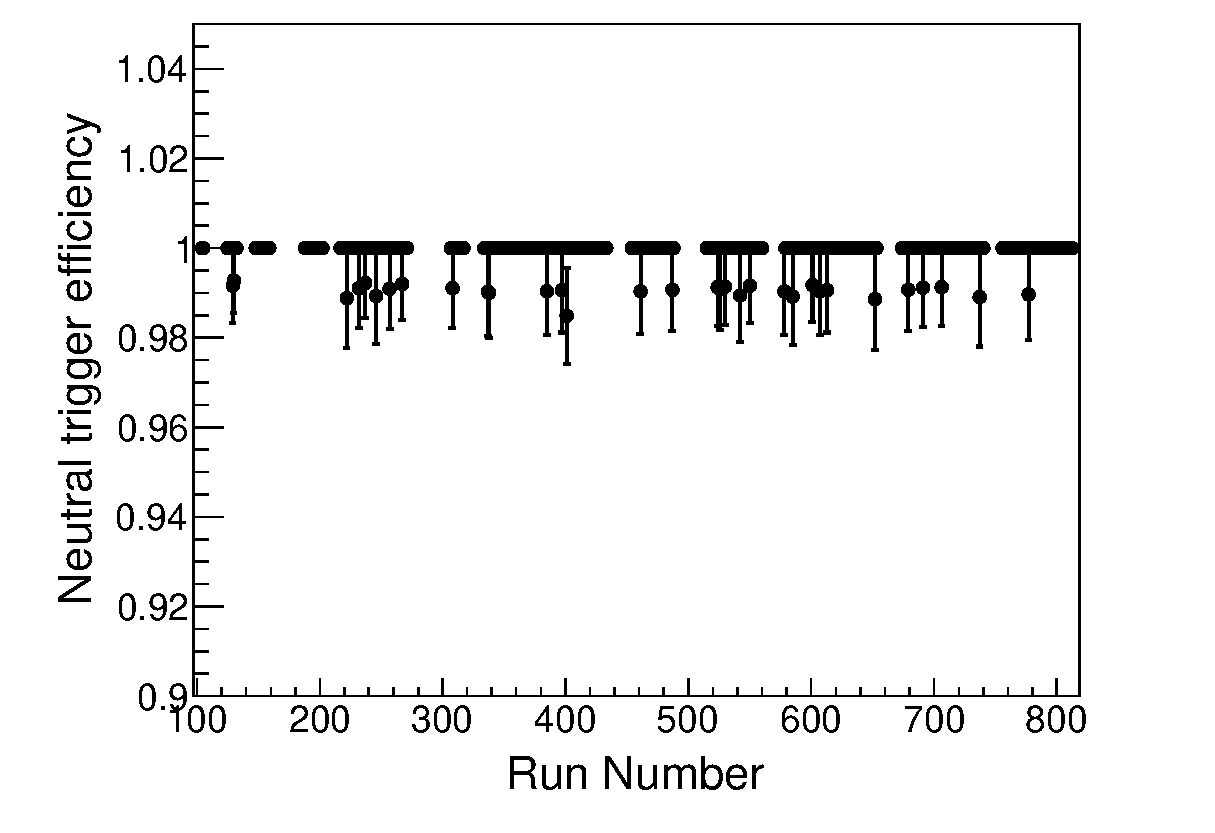
\includegraphics[width=5cm]{../pic/Run78/trigger/Neutral.eps}
    \end{minipage}
  \end{tabular}
  \caption{
    These figures show about trigger efficiencies in each run.
    The $d(K^-, p)$ analysis was analyzed using MR-RUN68 data which is shown in the above.
    The right above shows the K $\otimes$ CDH1 trigger and the left above shows the charge trigger.
    The $d(K^-, n)$ analysis was analyzed using MR-RUN78 data which is shown in the down.
    The right down shows the K $\otimes$ CDH1 trigger and the left down shows the neutral trigger.
  }
  \label{fig:trigger_eff}
\end{figure}

A trigger signal has the efficiency to actually output a signal when it should be output.
They are evaluated with more unbiased trigger conditions.
For example, in the case of a CDH 1hit trigger, if there is one or more hits in CDH among the data acquired by the Kaon beam trigger, check whether the CDH 1hit trigger signal is output.
Forward neutral and forward charged triggers are evaluated using data taken with $K\otimes CDH1$ trigger.
These are also evaluated for each run, as shown in Fig.\ref{fig:trigger_eff}.
For the forward proton $d(K^-, p)$, we are analyzing the MR-RUN69 data, which is shown in the above figure.
The figure on the right is the CDH1 trigger, and the figure on the left is the charge trigger.
For the forward neutron $d(K^-, n)$, we are analyzing the MR-RUN78 data, which is shown in the bottom figure.
The figure on the right is the CDH1 trigger, and the figure on the left is the neutral trigger.
